% DO NOT COMPILE THIS FILE DIRECTLY!
% This is included by the other .tex files.
\section*{Background}
\begin{frame}[t,plain]
\titlepage
\end{frame}
%%%%%%%%%%%%%%%%%%%%%%%%%%%%%%%%%%
%%%%%%%%%%%%%%%%%%%%%%%%%%%%%%%%%%
\begin{frame}{Plan for today}
 \begin{itemize}
  \item A brief overview of how we came to using phylogenetic trees and mathematical models;
  \item The awesome things we can do with them;
  \item An interesting combinatorics problem on how to build better trees.
 \end{itemize}
\end{frame}
%%%%%%%%%%%%%%%%%%%%%%%%%%%%%%%%%%
%%%%%%%%%%%%%%%%%%%%%%%%%%%%%%%%%%
\begin{frame}[t]{\textbf{In the beginning there were hierarchies...}}
 \begin{figure}[!h]
\begin{center}
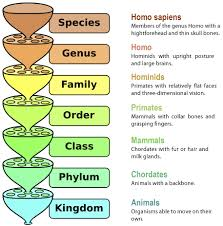
\includegraphics[scale=.55]{FIGURES/linnaeus_system.jpg}
\caption{Linnaean system of classification ($\sim 1735$)}
\end{center}
\end{figure}
\end{frame}
%%%%%%%%%%%%%%%%%%%%%%%%%%%%%%%%%%
%%%%%%%%%%%%%%%%%%%%%%%%%%%%%%%%%%
\begin{frame}[t]{\textbf{The plate tectonics of Biology...}}
\begin{columns}[c]
\column{2.5in}
\begin{figure}[!h]
\begin{center}
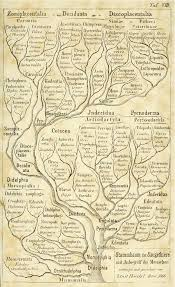
\includegraphics[scale=.55]{FIGURES/haeckel_tree_1866.jpg}
\caption{Haeckel (1866)}
\end{center}
\end{figure}
\column{2.5in}
\begin{itemize}
\item Darwin did not know how genetic variation arose or was transmitted;
\item Mendelian geneticists believed in evolutionary ``jumps'' and rejected natural selection;
\item Contrary to what is usually believed, Lamarckian thought was important to maintain gradualism;
\item[\tikzmark{bl}\textbullet] Haldane, Fisher and Wright reconciled population genetics and selection\footnote[1]{\tiny This is not the whole story!
Check the preface in~\cite{mayr1998}\\ for a much better account.}\tikzmark{br}
\end{itemize}
\tikz[overlay,remember picture]{\draw[white]
  ($(bl)+(-0.5em,0.9em)$) rectangle
  ($(br)+(2.5em,-0.3em)$);}
\end{columns}
\end{frame}
%%%%%%%%%%%%%%%%%%%%%%%%%%%%%%%%%%
%%%%%%%%%%%%%%%%%%%%%%%%%%%%%%%%%%
\begin{frame}[t]{\textbf{I've never done anything useful...}}
\begin{columns}[c]
\column{2.5in}
\begin{figure}[!h]
\begin{center}
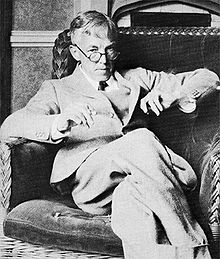
\includegraphics[scale=.55]{FIGURES/GHHardy.jpg}
\caption{Geoffrey Harold Hardy (1877-1947)}
\end{center}
\end{figure}
\column{2.5in}
\begin{itemize}
\item ``I have never done anything 'useful'.
No discovery of mine has made, or is likely to make, directly or indirectly, for good or ill, the least difference to the amenity of the world.''\footnote{\tiny\cite{titchmarsh1950}}
\item Oh yeah?\pause
\item[\tikzmark{bl}\textbullet]
\begin{align*}
A(p); a(q) \\
p + q &= 1 \\
p^2 + 2pq + q^2 &= 1 
\end{align*}
\tikzmark{br}\pause
\item Stability!
\end{itemize}
\tikz[overlay,remember picture]{\draw[green]
  ($(bl)+(-0.5em,0.9em)$) rectangle
  ($(br)+(17.0em,-0.3em)$);}
\end{columns}
\end{frame}
%%%%%%%%%%%%%%%%%%%%%%%%%%%%%%%%%%
%%%%%%%%%%%%%%%%%%%%%%%%%%%%%%%%%%
\begin{frame}{Population Genetics}
 \begin{itemize}[label={$\bullet$}]
 \item Hardy-Weinberg is nice and useful, but describes an ideal setting with no mutation, selection or population structure.
 \item In the 1980s, John Kingman starts a revolution...
\end{itemize}
\begin{figure}
 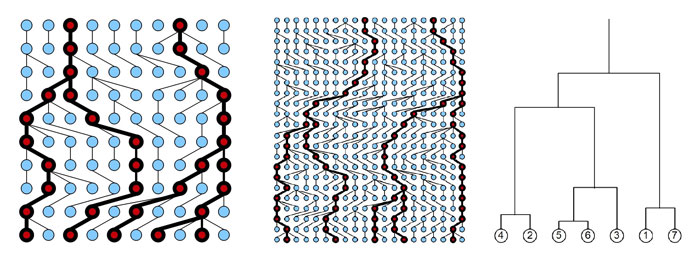
\includegraphics[scale=0.45]{FIGURES/kingman.jpg}
 \caption{Kingman's coalescent (1982)\footnote{\tiny Figure from~\url{http://culturemath.ens.fr/content/genealogie-de-populations-le-coalescent-de-kingman-2101}}}
\end{figure}
\end{frame}
%%%%%%%%%%%%%%%%%%%%%%%%%%%%%%%%%%
%%%%%%%%%%%%%%%%%%%%%%%%%%%%%%%%%%
\begin{frame}{Population Genetics}
\begin{columns}
 \column{2.5in}
\begin{figure}[!h]
\begin{center}
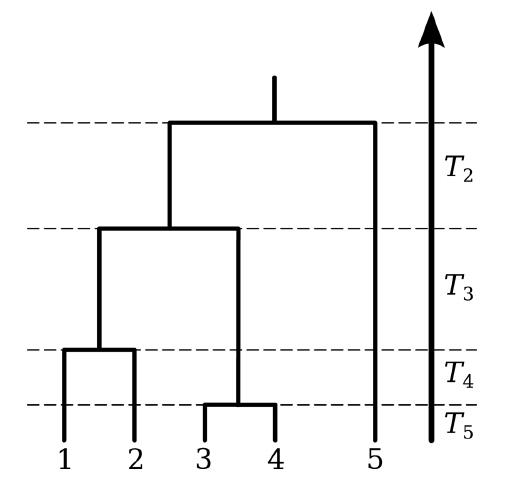
\includegraphics[scale=.45]{FIGURES/coaltimes.jpg}
\caption{Figure 4 from~\cite{volz2013}}
\end{center}
\end{figure}
 \column{2.5in}
 Let $T_n$ denote the time for $n$ lineages to~\textit{coalesce}, i.e., merge into one ancestral lineage, in a population of size $N$.
 Then:
\begin{align*}
Pr(T_n = t) &= \lambda_n e^{-\lambda_nt}\\
\lambda_n &= \binom{n}{2}\frac{1}{N} = \binom{n}{2}\frac{1}{N_e\tau}
\end{align*}
where $N_e$ is the effective population size and $\tau$ is the generation time.
Let $T_{\text{mrca}}$ denote the age of the most recent common ancestor:
\begin{align*}
 \mathbb{E}[T_{\text{mrca}}] &= \mathbb{E}[T_n] + \mathbb{E}[T_{n-1}] + \ldots + \mathbb{E}[T_2]\\
 &= 1/\lambda_n + 1/\lambda_{n-1} + \ldots + 1/\lambda_2\\
 &= 2N(1-\frac{1}{n})
\end{align*}

\end{columns}
\end{frame}
%%%%%%%%%%%%%%%%%%%%%%%%%%%%%%%%%%
%%%%%%%%%%%%%%%%%%%%%%%%%%%%%%%%%%
\section*{Phylodynamics}
\begin{frame}{Bridging Disease Ecology and Genetics}
% The fundamental idea of Phylodynamics is:
if the tree is a reasonable representation of ancestry, then we can use it as proxy to hidden/unobservable population processes.
One such process is infection:
\begin{align*}
 \frac{dS}{dt} &= -\beta I S \\
 \frac{dI}{dt} &=  \beta I S - \gamma I\\
 \frac{dR}{dt} &=  \gamma I.
\end{align*}
Here is an idea\footnote{\tiny Equations and ideas taken from~ \cite{volz2013}}:
\begin{equation*}
 \lambda_n(t) = \binom{n}{2}\frac{2\beta S(t)}{I(t)}
\end{equation*}
Some more glossing over the details yields:
\begin{equation*}
 \lambda_n = \binom{n}{2}\frac{2\gamma}{I}
\end{equation*}
\end{frame}
%%%%%%%%%%%%%%%%%%%%%%%%%%%%%%%%%%
%%%%%%%%%%%%%%%%%%%%%%%%%%%%%%%%%%
\begin{frame}{Bridging Disease Ecology and Genetics}
\begin{columns}
\column{2.5in}
\begin{figure}
  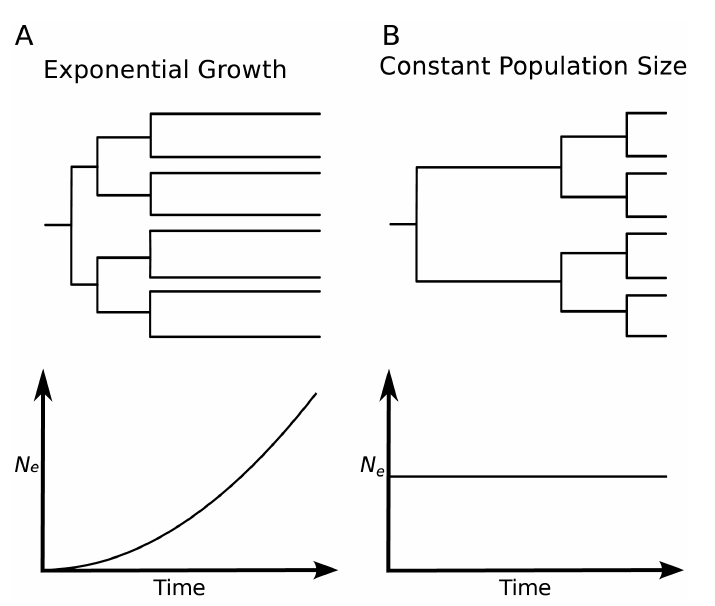
\includegraphics[scale=0.35]{FIGURES/pop_growth.jpg}
\end{figure}
\column{2.5in}
\begin{figure}
  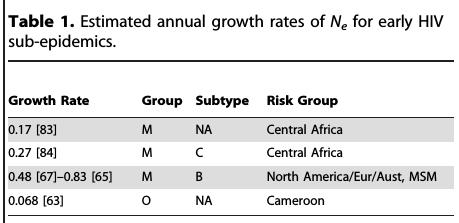
\includegraphics[scale=0.45]{FIGURES/hiv_growth.jpg}
  \caption{Taken from~\cite{volz2013}}
\end{figure}
\end{columns}
\end{frame}
%%%%%%%%%%%%%%%%%%%%%%%%%%%%%%%%%%
%%%%%%%%%%%%%%%%%%%%%%%%%%%%%%%%%%
\begin{frame}{Bridging Disease Ecology and Genetics II}
\begin{columns}
\column{2.5in}
\begin{figure}[!h]
\begin{center}
% \subfigure[]{
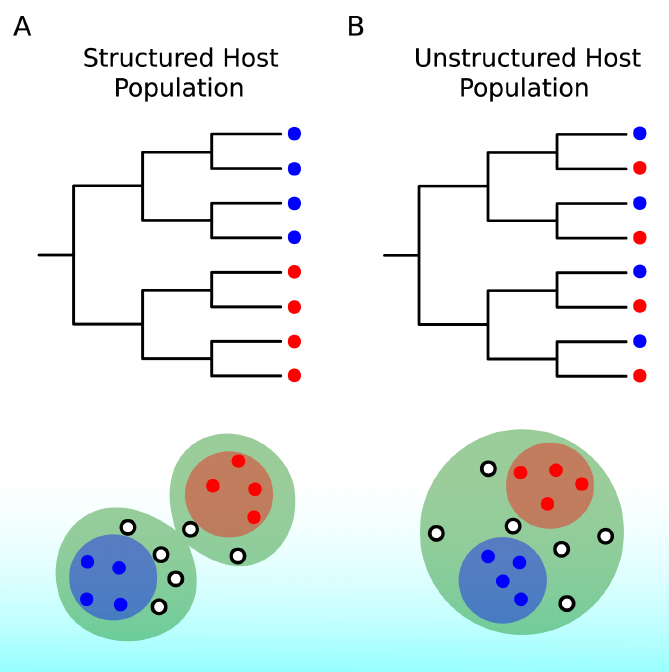
\includegraphics[scale=.23]{FIGURES/pop_structure.jpg} \\
% }
% \subfigure[]{
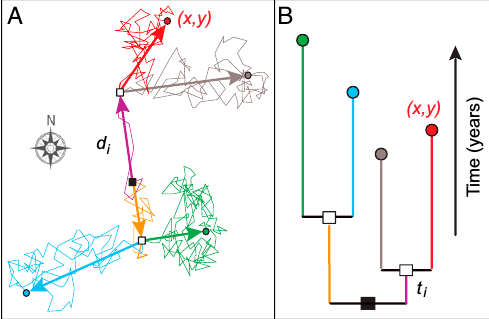
\includegraphics[scale=.4]{FIGURES/bmotion_phylo.jpg}
% }
\end{center}
\end{figure}
\column{2.5in}
Let $\mathbf{X}(t)$ be the state at the $t$.
We are interested in the likelihood of ending up in $\mathbf{X}(t)$ if we started at $\mathbf{X}(s)$.
Here's an idea~\citep{lemey2010}:
\begin{equation*}
 p(\mathbf{X}(t)|\mathbf{X}(s)) \sim MVN(\mathbf{X}(s), \mathbf{P}^{-1}\times(t-s))
\end{equation*}
where $\mathbf{P}$ is the infinitesimal precision matrix of the diffusion process.
Note that:\\
(i) the diffusion matrix depends only on time differences and;\\
(ii) analytical solutions are available through clever traversing of the tree~\citep{pybus2012}.
\end{columns}
\end{frame}

%%%%%%%%%%%%%%%%%%%%%%%%%%%%%%%%%%
%%%%%%%%%%%%%%%%%%%%%%%%%%%%%%%%%%
\begin{frame}{Bridging Disease Ecology and Genetics II}
``...phylogenies reconstructed from spatial epidemics
are branching structures that record the correlated histories of
transmission among sampled infections...''~\citep{pybus2012}
\begin{center}
\begin{figure}
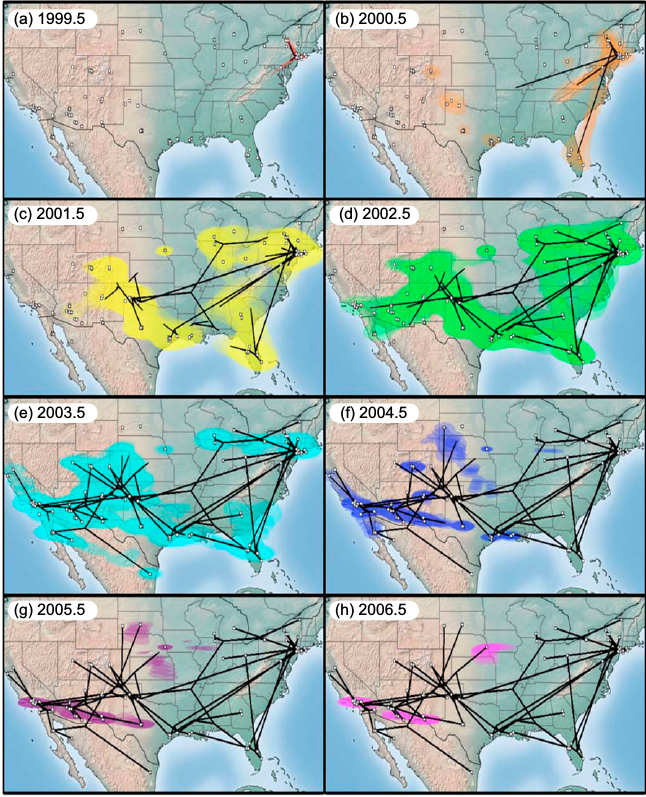
\includegraphics[scale=0.28]{FIGURES/wnv_usa.jpg}
 \caption{\scriptsize The spread of West Nile virus (WNV) in the US~\citep{pybus2012}}
\end{figure}
\end{center}
\end{frame}
%%%%%%%%%%%%%%%%%%%%%%%%%%%%%%%%%%
%%%%%%%%%%%%%%%%%%%%%%%%%%%%%%%%%%
\begin{frame}{Summary so far...}
\begin{itemize}
 \item By conditioning on the inferred ancestry of DNA/RNA sequences, we can use phylogenetic trees as correlation structures;
 \item It is possible to obtain insight into temporal (dynamic) and spatial features of populations from genetic data;
 \item \textcolor{green}{Phylogenies} are  the centre of it all: almost everything we do is \textcolor{green}{conditional} on the tree.\pause
 \item This suggests we should also pay close attention to tree estimation...
 Bayesian and maximum likelihood phylogenetic methods rely on stochastic tree search. There is great interest in making the \textcolor{red}{traversal} of tree-space more \textcolor{red}{efficient}.
\end{itemize}
\end{frame}
%%%%%%%%%%%%%%%%%%%%%%%%%%%%%%%%%%
%%%%%%%%%%%%%%%%%%%%%%%%%%%%%%%%%%
\section*{An open problem}
\begin{frame}{An open problem -- preliminaries}
\textbf{Defn. 1}: An (unrooted) phylogenetic $X$-tree is a tree $T$ on a tip (leaf) set $X$ with all internal nodes of degree of at least $3$.
If the degree of all internal nodes is exactly $3$ then we say we have a \textit{binary} $X$-tree. 
\begin{itemize}
 \item Every unrooted (rooted) binary $X$-tree has $2n - 3$ ($2n - 2$) edges (also called branches), with $n = |X|$;
 \item There exist $\frac{(2n-3)!}{2^{n-2}(n-2)!} = (2n-3)!!$ rooted $X$-trees on $n$ tips/leafs.
For $n = 53$, there are roughly as many trees as there are particles in the observable universe!
\end{itemize}
See~\cite{steel2014} for a gentle introduction to phylogenetic trees, specially targeted at mathematicians.
\end{frame}
%%%%%%%%%%%%%%%%%%%%%%%%%%%%%%%%%%%
%%%%%%%%%%%%%%%%%%%%%%%%%%%%%%%%%%%
\begin{frame}{Tree surgery...}
Let $Y \subset X$. Then call $X'$ the $Y$-tree that has internal nodes compatible with those in $T$, i.e., $X'$ is a \textit{subtree} of $X$.
An subtree-prune and re-graft (SPR) operation on a tree $T$ detaches $X'$ and re-grafts it onto another node in the tree.
\begin{center}
 \begin{figure}
  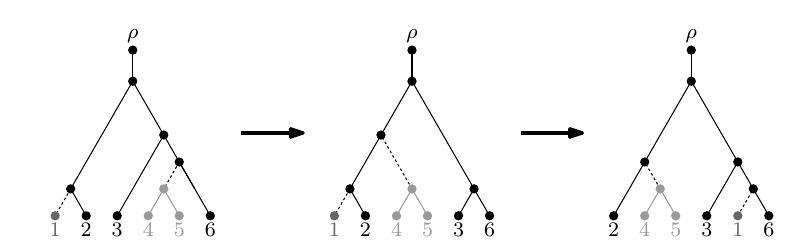
\includegraphics[scale=0.5]{FIGURES/two_sprs.jpg}
  \caption{Two consecutive (rooted) SPR operations on a 6-leaf tree~\citep{whidden2015}}
 \end{figure}
\end{center}
\end{frame}
%%%%%%%%%%%%%%%%%%%%%%%%%%%%%%%%%%%
%%%%%%%%%%%%%%%%%%%%%%%%%%%%%%%%%%%
\begin{frame}{Graphs about graphs...}
 \begin{center}
  \begin{figure}
   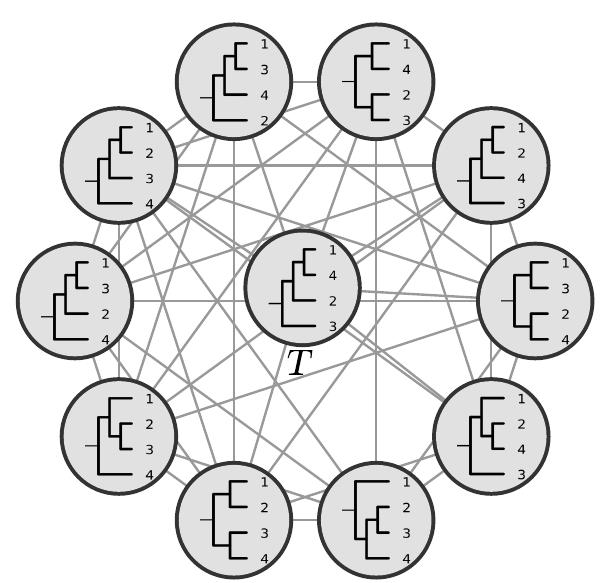
\includegraphics[scale=0.35]{FIGURES/spr_graph.jpg}
   \caption{The neighbourhood of $T$ in the SPR graph ($G(n)$)~\citep{whidden2015}}
  \end{figure}
   The diameter is \textcolor{red}{$n - \Theta(\sqrt{n})$} and the average degree is \textcolor{red}{$2(n-3)(2n-7)$}.
 \end{center}
\end{frame}
%%%%%%%%%%%%%%%%%%%%%%%%%%%%%%%%%%%
%%%%%%%%%%%%%%%%%%%%%%%%%%%%%%%%%%%
\begin{frame}{Ricci-Ollivier curvature~\citep{whidden2015}}
 With a random-walk in a metric space, we can define ``curvature'', that is, how ``difficult'' it is to go from $x$ to $y$~\citep{ollivier2009} as follows:
%  \cite{whidden2015} consider two points $x$ and $y$ on the SPR graph ($G$).
 let $m_x$ and $m_y$ be the probability masses of the positions $x$ and $y$ on $G(n)$ after some (finite) time. Then:
 \begin{equation}
 W_1(m_x, m_y) := \min_{\xi \in \Pi(m_x, m_y)} \sum_{\{z,w\} \subset V} d(z,w) \xi(z,w)
 \end{equation}
% which loosely measures how much ``work'' is involved in moving $m_x$ to $m_y$ along $G$.
The so-called coarse Ricci-Ollivier curvature of $x$ and $y$ is then:
\begin{equation}
\kappa(m; x, y) := 1 - \frac{W_1(m_x, m_y)}{d(x, y)}.
\end{equation}
Here, for two trees $T$ and $S$, $d(T,S)$ is how many SPR operations are needed to transform $T$ in $S$ (vice-versa). 
\end{frame}
%%%%%%%%%%%%%%%%%%%%%%%%%%%%%%%%%%%%
%%%%%%%%%%%%%%%%%%%%%%%%%%%%%%%%%%%
\begin{frame}{A conjecture}
 \cite{whidden2015} prove a bunch of useful results about the SPR graph.
 For instance, they show that for two trees $T$ and $S$:
 \begin{equation}
 \frac{-2}{d(T,S)} \le \kappa(T,S) \le \frac{2}{d(T,S)}
 \end{equation}
 Moreover, if $T$ and $S$ are adjacent (with $|T| = |S| = n$), the the maximum curvature of the uniform random-walk is 
 \begin{equation}
  \frac{6n-17}{3n^2-13n+14}
 \end{equation}
\textit{Conjecture~\citep{whidden2015}: Let $k_n$ be the maximum curvature between two trees with $n$-leaves.
	Then:
	\begin{equation}
	 k_n \le \frac{2}{D(n)-1}
	\end{equation}
}
where $D(n)$ is the diameter of the SPR graph on $n$-leaves trees.
\end{frame}
%%%%%%%%%%%%%%%%%%%%%%%%%%%%%%%%%%%
%%%%%%%%%%%%%%%%%%%%%%%%%%%%%%%%%%%
\begin{frame}{My two pence}
 \begin{itemize}
  \item It is important to prove not only this conjecture, but also to study variants on different spaces resulting from other transformations;
  \item In the context of phylodynamics, height-restricted SPRs are arguably a more important transformation;
  \item Recursive application of the techniques used to prove the curvature for adjacent trees could be extended to k-radius neighbourhoods;
  \item A more productive approach could be to relate what we know for the graph (e.g. average degree, diameter, etc) to its local properties, taking advantage of more heavy graph-theoretic methods/results.
 \end{itemize}
\end{frame}
%%%%%%%%%%%%%%%%%%%%%%%%%%%%%%%%%%%
%%%%%%%%%%%%%%%%%%%%%%%%%%%%%%%%%%%
\begin{frame}{Wrap-up}
 \begin{itemize}
  \item Maths was fundamental to advance our understanding of population genetics;\pause
  \item Maths plays a central role in Phylodynamics, be it on developing models or figuring out how to fit them;\pause
  \item There is a lot of cool maths to be done in:\pause
  \begin{itemize}
   \item Lie algebras of Markov models of DNA evolution;
   \item Further merging ODE-based models and phylogenetics;
   \item[\tikzmark{bl}\textbullet] Combinatorics on the space of phylogenetics trees~\sout{and networks}!\tikzmark{br}
  \end{itemize}
  \tikz[overlay,remember picture]{\draw[red]
  ($(bl)+(-0.5em,0.9em)$) rectangle
  ($(br)+(1.0em,-0.3em)$);}\pause
  \item Maths rocks! Q.E.D
 \end{itemize}
\end{frame}
%%%%%%%%%%%%%%%%%%%%%%%%%%%%%%%%%%%
%%%%%%%%%%%%%%%%%%%%%%%%%%%%%%%%%%%
\begin{frame}{Thank you!}
\begin{itemize}
 \item Thanks a bunch for watching!
 \item I am grateful to the organising committee for the invitation;
 \item Special thanks to Andrew Rambaut (Edinburgh), \underline{Mike Steel} (Cantenbury, NZ), Patrice Showers Corneli (Utah), \underline{Erick Matsen} (Hutchson) and \underline{Felipe Figueiredo} (PROCC)\footnote{Mathematicians are underlined.}.
\end{itemize}
\end{frame}
%%%%%%%%%%%%%%%%%%%%%%%%%%%%%%%%%%%%
%%%%%%%%%%%%%%%%%%%%%%%%%%%%%%%%%%%%